\chapter{Image representation and description}

\section{Problem statement}

\begin{enumerate}[(a)]

    \item Develop a program to implement the boundary following
    algorithm, the resampling grid and calculate the chain code and
    the first difference chain code. Use the image ‘noisy\_stroke.tif’ for
    test. (For technique details, please refer to pp.818-822 (3rd
    edition, Gonzalez DIP) or boundaryfollowing.pdf at the same
    address of the slides.)

    \item Develop a program to implement the image description
    by the principal components (PC). Calculate and display the PC
    images and the reconstructed images from 2 PCs. Use the six
    images in ‘washingtonDC.rar’ as the test images.

\end{enumerate}

\section{Python implementation}
\bigskip
Four programs: \\
\begin{itemize}
    \item Boundary following: \textbf{boundary.py}

    Usage:~\textbf{boundary.py [-h] [--smooth] image\_path}\\
    Use \textbf{python boundary.py -h} to see the help.

    \bigskip
    \item Resampling grid: \textbf{resampling.py}

    Usage:~\textbf{resampling.py [-h] [-s SAMPLING [SAMPLING ...]] boundary\_image}\\
    Use \textbf{python resampling.py -h} to see the help.

    \bigskip
    \item Chain code: \textbf{chaincode.py}

    Usage:~\textbf{chaincode.py [-h] [-s SAMPLING [SAMPLING ...]] boundary\_image}\\
    Use \textbf{python chaincode.py -h} to see the help.

    \bigskip
    \item Image description by the principal components (PC): \textbf{pc.py}

    Usage:~\textbf{pc.py [-h] [-n N] [--debug] [--diff] [--nshow]}\\
    Use \textbf{python pc.py -h} to see the help.

\end{itemize}

\pagebreak

\section{Boundary following}

\textbf{python boundary.py noisy\_stroke.tif}.

\begin{figure}[!htb]\centering
    \begin{minipage}{0.45\textwidth}
        \frame{
\includegraphics[width=\linewidth]{./images/10/noisy_stroke.png}}
        \caption{\small{Original image}}
    \end{minipage}
    \begin{minipage}{0.45\textwidth}
        \frame{
\includegraphics[width=\linewidth]{./images/10/noisy_stroke_b_w.png}}
        \caption{\small{Black \& white}}
    \end{minipage}
\end{figure}

\begin{figure}[!htb]\centering
    \begin{minipage}{0.7\textwidth}
        \frame{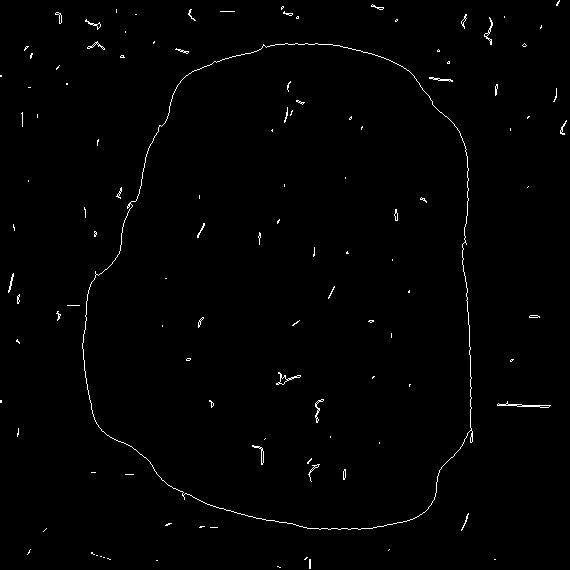
\includegraphics[width=\linewidth]{./images/10/noisy_stroke_b_w_boundary.png}}
        \caption{\small{Boundaries}}
    \end{minipage}
\end{figure}

Even the boundaries of the noise are found\ldots We need to remove the noise beforehand. For that, let use a Gaussian blur of mean $0$ and variance $10$.

\pagebreak

\textbf{python boundary.py noisy\_stroke.tif --smooth}.

\begin{figure}[!htb]\centering
    \begin{minipage}{0.45\textwidth}
        \frame{
\includegraphics[width=\linewidth]{./images/10/noisy_stroke.png}}
        \caption{\small{Original image}}
    \end{minipage}
    \begin{minipage}{0.45\textwidth}
        \frame{
\includegraphics[width=\linewidth]{./images/10/noisy_stroke_smoothing_s10_b_w.png}}
        \caption{\small{Smoothing + binarisation}}
    \end{minipage}
\end{figure}

\begin{figure}[!htb]\centering
    \begin{minipage}{0.7\textwidth}
        \frame{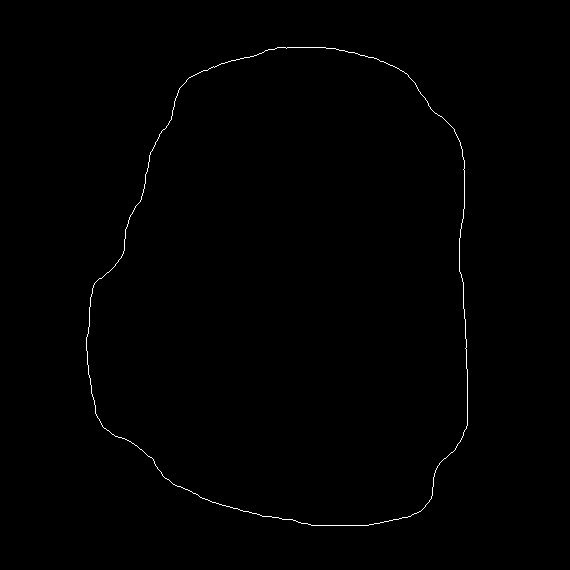
\includegraphics[width=\linewidth]{./images/10/noisy_stroke_boundary.png}}
        \caption{\small{Boundaries}}
    \end{minipage}
\end{figure}


\pagebreak

\section{Resampling grid}

\textbf{python resampling.py noisy\_stroke\_boundary.png -s Sx Sy}, where $Sx$ and $Sy$ are the sampling intervalles along the X and Y axis.

\begin{figure}[!htb]\centering
    \begin{minipage}{0.45\textwidth}
        \frame{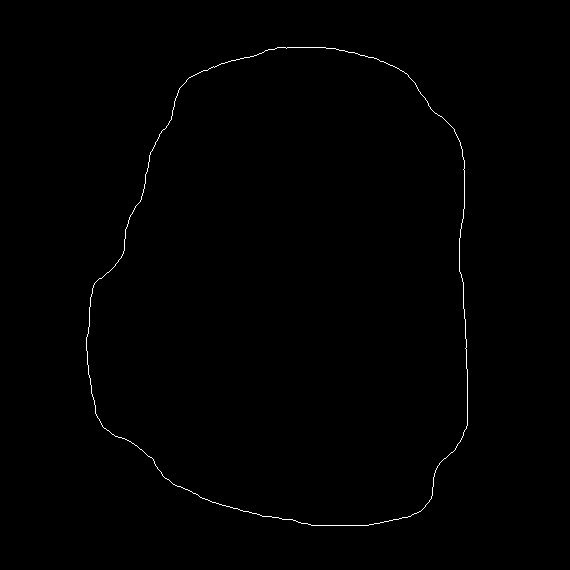
\includegraphics[width=\linewidth]{./images/10/noisy_stroke_boundary.png}}
        \caption{\small{Original image}}
    \end{minipage}
    \begin{minipage}{0.45\textwidth}
        \frame{
\includegraphics[width=\linewidth]{./images/10/noisy_stroke_resampling_grid_10.png}}
        \caption{\small{R-grid (S = (10, 10))}}
    \end{minipage}
\end{figure}

\begin{figure}[!htb]\centering
    \begin{minipage}{0.45\textwidth}
        \frame{
\includegraphics[width=\linewidth]{./images/10/noisy_stroke_resampling_grid_30.png}}
        \caption{\small{R-grid (S = (30, 30))}}
    \end{minipage}
    \begin{minipage}{0.45\textwidth}
        \frame{
\includegraphics[width=\linewidth]{./images/10/noisy_stroke_resampling_grid_5_30.png}}
        \caption{\small{R-grid (S = (5, 30))}}
    \end{minipage}
\end{figure}

\pagebreak
\section{Chain code and first difference chain code}

\subsection{Chain code - resampling grid (10, 10)}

\begin{figure}[!htb]\centering
    \frame{
\includegraphics[width=0.8\linewidth]{./images/10/noisy_stroke_resampling_grid_10.png}}
    \caption{\small{Resampling grid (S = (10, 10))}}
\end{figure}
Chaincode (length = 170):
\begin{center}
00000060000600706606060606606666666\\
66466660666666666666666664646466656\\
44464444444444244444344424424424224\\
24424424222224222222202220022022220\\
202222202202022220200200020002
\end{center}

\bigskip

First difference (length = 169):
\begin{center}
00000620006207160262626260260000000\\
06200026000000000000000062626200716\\
00260000000006200007100620620626026\\
20620626000026000000620060206200062\\
62000062062620006260260026002
\end{center}

\pagebreak
\subsection{Chain code - resampling grid (30, 30)}

\begin{figure}[!htb]\centering
    \frame{
\includegraphics[width=0.8\linewidth]{./images/10/noisy_stroke_resampling_grid_30.png}}
    \caption{\small{Resampling grid (S = (30, 30))}}
\end{figure}

Chaincode (length = 56):
\begin{center}
00060606066666666666466444444344242422422022022202220020
\end{center}

\bigskip

First difference (length = 55):
\begin{center}
0062626260000000000620600000710626260260620620062006026
\end{center}


\pagebreak

\section{Principal components}

\textbf{python pc.py --diff -n 2}

%\begin{figure}[!htb]\centering
    %\begin{minipage}{0.45\textwidth}
        %\frame{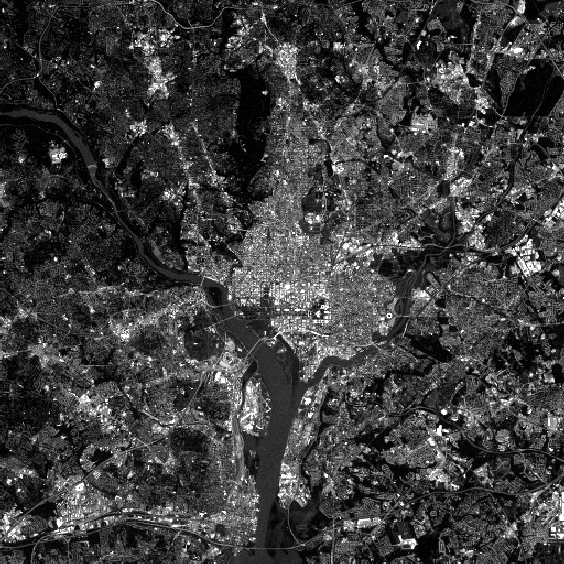
\includegraphics[width=\linewidth]{./images/10/band1.png}}
        %\caption{\small{Band 1}}
    %\end{minipage}
    %\begin{minipage}{0.45\textwidth}
        %\frame{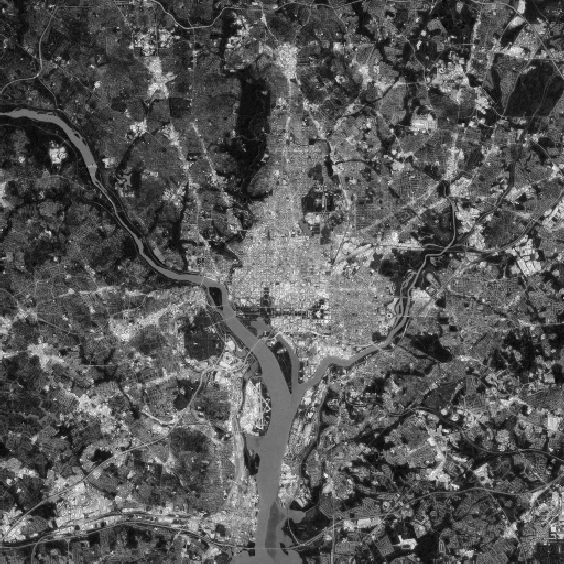
\includegraphics[width=\linewidth]{./images/10/pc_eigen2_band1.png}}
        %\caption{\small{Band 1 reconstructed}}
    %\end{minipage}
%\end{figure}

%\begin{figure}[!htb]\centering
    %\begin{minipage}{0.7\textwidth}
        %\frame{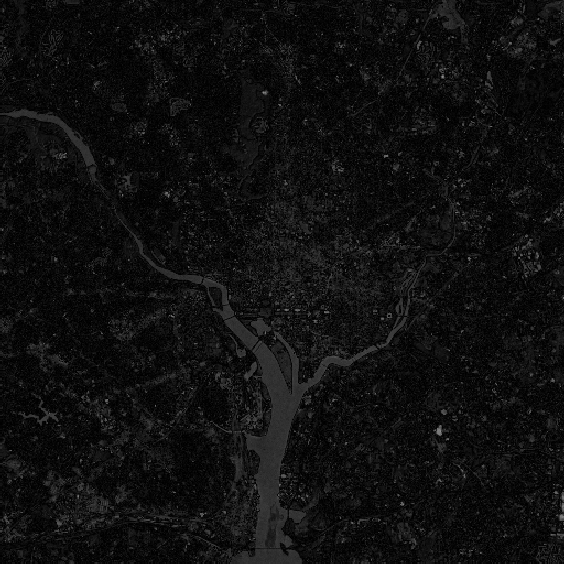
\includegraphics[width=\linewidth]{./images/10/pc_eigen2_band1_diff.png}}
        %\caption{\small{Band 1 difference}}
    %\end{minipage}
%\end{figure}

\pagebreak
